
%% Meta: Diagramme Lesen
%%

\input{bmsLayoutPage}

\renewcommand{\metaHeaderLine}{Arbeitsblatt}
\renewcommand{\arbeitsblattTitel}{Diagramme Lesen (V 0.1)}

%%%%%%%%%%%%%%%%%%%%%%%%%%%%%%%%%%%%%%%%%%%%%%%%%%%%%%%%%%%%%%%%%%

%\usepackage{amssymb} 
%\usepackage{cancel}

%\newcommand\Ccancel[2][black]{\renewcommand\CancelColor{\color{#1}}\cancel{#2}}


\begin{document}%%
\arbeitsblattHeader{}


\section*{Bergiffsammlung}
Die Datenanalyse beinhaltet diverse mehr oder weniger einfache Themen. Doch damit das ganze übersichtlich bleibt, erstellen Sie sich eine Mindmap und eine Liste mit den wichtigsten Begriffen.

Vorschläge:

\begin{itemize}
\item Kärtchen
\item Heft
\item Quizlet
\item Elektronische/Physische Dokumente
\item Wiki
\item ...
\end{itemize}

Eine Sammlung der wichtigsten Begriffe finden Sie im OLAT im \href{https://olat.bms-w.ch/auth/RepositoryEntry/5242983/path%3DIndex/0}{Wiki}.

\newpage
\section{Datenerhebung}
\subsection{Erhebungstechniken}\
Entscheiden Sie bei den folgenden Statistiken, um welche der vier Erhebungstechniken (Experiment, Befragung, Beobachtungsstudie, Datensammlung) es 
sich dabei handelt. Bei Mischformen oder möglichen "Doppellösungen"
wählen Sie die offensichtlichste. \TRAINER{}

\begin{enumerate}
\item
Um herauszufinden, ob ein neues Waschmittel Flecken besser entfernt, werden 20 identische T-Shirts mit Rotwein beschmutzt.
    Die eine Hälfte wird mit dem neuen Mittel gewaschen, die andere Hälfte mit einem herkömmlichen Produkt.
    Danach wird der Sauberkeitsgrad verglichen. \TRAINER{Experiment: Aktiver Eingriff (Manipulation der Variable "Waschmittel") und Vergleichsgruppe.}

\item
Ein Mitarbeiter eines Marktforschungsinstituts ruft zufällig ausgewählte Haushalte an und bittet die Personen am Telefon,
    ihre Meinung zu verschiedenen Käsesorten auf einer Skala von 1 bis 5 zu äußern. \TRAINER{Befragung: Direkte Auskunftserteilung durch Personen (Telefoninterview).}

\item
Ein Biologe sitzt versteckt in einem Tarnzelt am Seeufer und führt eine Strichliste darüber, welche Entenarten wie oft am
    Tag den Uferbereich zur Gefiederpflege aufsuchen. \TRAINER{Beobachtung	Passives Erfassen von natürlichem Verhalten ohne Beeinflussung.}

\item
Ein Versicherungsmathematiker nutzt die digitalen Archivbestände seiner Firma, um die Schadensfälle der letzten
    30 Jahre nach Regionen auszuwerten. \TRAINER{Datensammlung	Rückgriff auf bereits vorhandene Bestände (Sekundärdaten).}

\item
Eine Softwareentwicklerin möchte wissen, welches Button-Design besser funktioniert. Die Website zeigt der einen Hälfte
    der Nutzer einen grünen Knopf und der anderen Hälfte einen blauen Knopf. Das System misst automatisch, welcher
    Knopf häufiger angeklickt wird. \TRAINER{Datensammlung	Rückgriff auf bereits vorhandene Bestände (Sekundärdaten).}

\item
Nach einem Kinofilm werden die Besucher am Ausgang gebeten, ein kurzes Formular auszufüllen, in dem sie angeben,
    wie ihnen die Handlung und die schauspielerische Leistung gefallen haben. \TRAINER{Befragung: Schriftliche Selbstauskunft der Kinobesucher.}

\item
Ein Verkehrsplaner stellt eine Kamera an einer vielbefahrenen Kreuzung auf. Später zählt er am Bildschirm aus,
    wie viele Fahrzeuge die Busspur unerlaubt nutzen, ohne dass die Fahrer davon wissen. \TRAINER{Beobachtung: Erfassen von Ereignissen (Verkehrsfluss) in der Realität.}

\item
Eine Historikerir analysiert die Geburts- und Sterberegister einer Stadtgemeinde aus dem 19. Jahrhundert, um die
    damalige durchschnittliche Lebenserwartung zu berechnen. \TRAINER{Datensammlung	Nutzung historischer Register/Archive.}

\item
In einer Studie soll geprüft werden, ob klassische Musik beim Lernen hilft. Eine Gruppe von Schülern lernt
    Vokabeln bei Mozart-Klängen, während eine andere Gruppe in absoluter Stille lernt. Die Vokabelkenntnisse werden
    anschließend geprüft. \TRAINER{Experiment: Gezielte Veränderung der Bedingungen (Musik vs. Stille).}

\item
Eltern erhalten von der Schulleitung einen Brief mit der Bitte, schriftlich mitzuteilen, wie viel Zeit ihre Kinder
    durchschnittlich pro Tag mit digitalen Medien verbringen. \TRAINER{Befragung	Auskunft über persönliches Verhalten per Fragebogen.}

\item
Ein Einzelhändler verfolgt über die Signale der Kunden-WLANs anonym, welche Wege die Käufer im Supermarkt
    nehmen und vor welchen Regalen sie am längsten stehen bleiben. \TRAINER{Beobachtung	Aufzeichnung von Laufwegen ohne Interaktion mit den Personen.}

\item
Ein Ökonom lädt die öffentlich zugänglichen Geschäftsberichte aller Unternehmen herunter, welche für den Swiss
    Market Index (SMI) verwendte werden , um die Gewinnentwicklung der letzten zehn Jahre zu vergleichen. \TRAINER{Datensammlung	Auswertung bereits veröffentlichter Berichte.}

\item
Ein Lebensmitteltechniker testet die Haltbarkeit von Milch bei unterschiedlichen Lagertemperaturen (5\degre{}C, 10\degre{}C und 15\degre{}C).
    Er misst täglich den Säuregehalt, wobei alle anderen Umgebungsfaktoren identisch bleiben. \TRAINER{Experiment	Systematische Variation der Temperatur unter Laborbedingungen.}

\item
Ein Student führt auf dem Campus kurze Interviews und fragt seine Kommilitonen direkt, wie viel Geld sie monatlich für Miete ausgeben. \TRAINER{Befragung	Mündliche Auskunft im direkten Kontakt.}

\item
Ein Meteorologe nutzt die Aufzeichnungen einer Wetterstation, die seit 1950 automatisch Temperatur und Niederschlag speichert, um einen Trend zur Erderwärmung nachzuweisen. \TRAINER{Datensammlung	Verwendung einer bestehenden Zeitreihe/Datenbank.}
\end{enumerate}



\newpage

\subsection{Fehlerarten}

Unterscheiden Sie in die Fehlerkategorien ...


\begin{itemize}
\item Zufällige Fehler (Messungenauigkeit)
\item Systematischer Fehler
\item Übertragungsfehler
\item Mutwilliger Fehler
\end{itemize}

\begin{enumerate}
\item 
 Beim Wiegen von Meerschweinchen für eine Biologiestudie zeigt die digitale Waage bei demselben Tier nacheinander 852 g, 855 g
     und 851 g an, obwohl sich das Tier kaum bewegt hat. \TRAINER{Zufälliger Fehler: Typische Messungenauigkeit/Schwankung der Hardware.}

\item
Eine Person tippt die Ergebnisse einer Umfrage in eine Excel-Tabelle ein. Dabei verrutscht sie in der Zeile und trägt den Wert 1.500
     in das Feld für das Alter ein, während die 25 (Jahre) im Feld für das Einkommen landet. \TRAINER{Übertragungsfehler	Klassischer Tippfehler durch Verrutschen in der Tabelle.}

\item
Um eine Studie schnell zu veröffentlichen, denkt sich ein Forschungsteam die fehlenden 20 Datensätze einfach aus, statt die fehlenden
     Personen tatsächlich noch zu befragen. \TRAINER{Mutwilliger Fehler:	Bewusste Erfindung von Daten (Fälschung).}

\item
Eine Person misst die Raumtemperatur mit einem Thermometer, das nicht korrekt kalibriert wurde und deshalb bei jeder Messung
     grundsätzlich 1,5 Grad zu viel anzeigt. \TRAINER{Systematischer Fehler:	Das Gerät ist falsch eingestellt (konstante Abweichung).}

\item
In einem Laborbericht wird der Eisenwert einer Pflanze notiert. Beim Abtippen für die Veröffentlichung wird das Komma jedoch um
     eine Stelle nach rechts verschoben, wodurch der Wert plötzlich zehnmal so hoch erscheint. \TRAINER{Übertragungsfehler	Schreibfehler (Kommafehler) bei der Datenaufbereitung.}

\item
Eine sportliche Leitung wertet einen Wettkampf aus. Da eine teilnehmende Person aus dem eigenen Verein stammt, wird deren
    Zeit bei der manuellen Zeitnahme absichtlich um zwei Zehntelsekunden nach unten korrigiert. \TRAINER{Mutwilliger Fehler:	Absichtliche Manipulation zugunsten einer Person.}

\item
Beim Ablesen eines analogen Messbechers schaut die Laborassistenz jedes Mal leicht schräg von oben auf die Skala,
    wodurch die Flüssigkeitsmenge immer etwas geringer protokolliert wird, als sie tatsächlich ist. \TRAINER{Systematischer Fehler:	Parallaxenfehler durch falsche Blickrichtung 
    (konstante Abweichung).}

\item
Eine Schiedsperson im Eiskunstlauf gibt einer befreundeten Person bewusst eine höhere Punktzahl in der B-Note,
    um deren Siegchancen zu erhöhen. \TRAINER{Mutwilliger Fehler:	Subjektive Begünstigung (Bias) durch die Schiedsperson.}

\item
In einer Wetterstation werden Windgeschwindigkeiten gemessen. Aufgrund von minimalen, unvorhersehbaren Luftverwirbelungen
    am Sensor schwanken die Werte bei eigentlich konstantem Wind ständig um ±0,2 km/h. \TRAINER{Zufälliger Fehler:	Unvermeidbare Umwelteinflüsse (Rauschen).}

\item
Eine Lehrkraft korrigiert einen Test und stellt am Ende fest, dass sie bei allen Schülerinnen bzw. Schülern der Klasse die letzte
    Aufgabe mit einem Punkt zu wenig bewertet hat. \TRAINER{Systematischer Fehler:	Ein konstanter Fehler, der alle Datensätze 
    gleichermaßen betrifft.}

\item
Beim Übertragen von handschriftlichen Notizen in den Computer wird die Ziffer „0“ fälschlicherweise als „8“ gelesen und so
    in die Statistik übernommen. \TRAINER{Übertragungsfehler	Lesefehler bei der Digitalisierung analoger Daten.}

\item
Ein Team möchte beweisen, dass ein neues Düngemittel wirkt. Daten von Pflanzen, die trotz Dünger kaum gewachsen sind,
    werden einfach gelöscht und nicht in die Endauswertung einbezogen. \TRAINER{Mutwilliger Fehler:	Selektive Datenauswahl („Cherry Picking“), um ein 
    Ergebnis zu erzwingen.}

\item
Bei einer Volkszählung wird ein Fragebogen von einem Stapel auf den anderen gelegt. Dabei wird die Rückseite übersehen und
    die Daten der dort eingetragenen drei Personen werden gar nicht erfasst. \TRAINER{Übertragungsfehler	Datenverlust durch Unachtsamkeit beim Sortieren.}

\item
Eine Person misst die Länge eines Tisches mit einem alten Holzlineal, dessen vordere Kante um 2 mm abgegriffen und kürzer ist.
    Jede Messung führt somit zu einem falschen Ergebnis. \TRAINER{Systematischer Fehler:	Beschädigtes Messwerkzeug führt zu immer
     gleichem Fehler.}

\item Bei einer Geschwindigkeitskontrolle der Polizei löst die Radarkamera aufgrund einer kurzzeitigen elektronischen
    Interferenz bei einem Auto aus, das eigentlich exakt die erlaubte Geschwindigkeit eingehalten hat. \TRAINER{Zufälliger Fehler:	Einmaliges technisches Versagen/Ausreißer ohne System.}

\end{enumerate}
\newpage
\subsection{Bias}

Erklären Sie, warum in den folgenden Erhebungen ein Bias (Stichprobenverzerrung)
vorliegt.

\begin{enumerate}
\item
Die Bibliotheks-Studie: Da im Juni die wichtigen Abschlussprüfungen anstehen, möchte die
    Universitätsleitung die durchschnittliche wöchentliche Lernzeit der Studierenden ermitteln.
    Die Kurzinventur der Anwesenden Lernenden findet im Mai in der Bibliothek statt, da das Personal in diesem Monat die wenigsten
    Feiertage hat und die Erfassung so am effizientesten durchgeführt werden kann. \TRAINER{Orts- und Zeit-Bias:
	Die Begründung (wenig Feiertage) klingt logisch,
 	lenkt aber davon ab, dass im Mai (kurz vor den Prüfungen) nur die fleißigsten
	Studierenden in der Bibliothek anzutreffen sind.
	Wer zu Hause oder gar nicht lernt, fehlt.
}

\item
    Die Service-Zufriedenheit: Ein Dienstleistungsunternehmen möchte die Zufriedenheit der
    Kundschaft mit der Beratung vor Ort ermitteln. Dazu wird in der Wartezone eine Postkarte bereitgelegt,
    die nach dem Termin auf freiwilliger Basis ausgefüllt und in eine Box geworfen werden kann. \TRAINER{Self-Selection Bias:
	Da die Teilnahme freiwillig ist, werden hauptsächlich Menschen mit 
	extremen Meinungen (sehr wütend oder sehr begeistert) mitmachen. 
	Die zufriedene Mehrheit wird ignoriert.}

\item
Die Senioren-Studie: Ein Forschungsprojekt untersucht die digitale Kompetenz von Seniorinnen
    und Senioren in Deutschland. Um eine möglichst hohe Reichweite in dieser Altersgruppe zu erzielen,
    wird eine Werbeanzeige auf Instagram geschaltet, die per Klick direkt zu einem Online-Fragebogen führt. \TRAINER{Medien-Bias:
	Seniorinnen und Senioren, die Instagram nutzen, sind bereits überdurchschnittlich
	digital kompetent. Die Studie erfasst also nur die "Digital-Profis" dieser Altersgruppe.}

\item
Die Zeitungs-Umfrage: Ein Verlag möchte wissen, wie hoch das Interesse an modernen, rein digitalen
    Nachrichtenangeboten in der Bevölkerung ist. Zu diesem Zweck wird in der Print-Version
    der Tageszeitung ein QR-Code mit einem Link zur Teilnahme an der Umfrage abgedruckt. \TRAINER{Medien-Bias
	Wer die Print-Version liest, gehört zur Zielgruppe, die traditionelle Medien bevorzugt.
	Die Meinung von Menschen, die bereits komplett auf Print verzichten,
	wird nicht gehört.}

\item
Die Work-Life-Balance: Ein Institut führt eine Telefonstudie zur Zufriedenheit mit der Work-Life-Balance
    bei Erwerbstätigen durch. Die Anrufe erfolgen vorrangig auf Festnetzanschlüssen an Werktagen in der
    Zeit zwischen 09:00 und 12:00 Uhr. \TRAINER{Verfügbarkeits-Bias:
	Wer vormittags unter einer Festnetznummer erreichbar ist,
	arbeitet oft im Homeoffice oder ist nicht voll erwerbstätig. Menschen in Berufen
	ohne Schreibtisch (Pflege, Bau, Handel) werden kaum erreicht.}

\newpage

\item
Das App-Feedback: Ein Softwareunternehmen analysiert die Qualität eines neuen Updates.
    Dabei werden vorzugsweise die Sterne-Bewertungen und schriftlichen Kommentare ausgewertet,
    welche die Nutzenden im offiziellen App-Store hinterlassen haben. \TRAINER{Polarisations-Bias
	App-Store-Bewertungen spiegeln selten den Durchschnitt
	wider. Meistens melden sich Nutzende dort nur bei Problemen (Frust) oder bei
	extremer Begeisterung zu Wort.}

\item
Um die Durchschnittliche Anzahl Kinder pro schweizer Familie zu erheben, werden alle 
    Schülerinnen bzw. Schüler der BMS-Winterthur befragt, wie viele Kinder Ihre Familie hat. \TRAINER{Abdeckungs-Bias:
	Schülerinnen bzw. Schüler ein und derselben Alterklasse 16 - 25 jährige
	repräsentieren nicht die gesamte Bevölkerung. Zudem ist nicht klar, ob ein Schüler,
	der selbst schon eigene Kinder hat, dies nun angeben soll, oder ob er sich und
	seine eigenen Geschwister zählen soll. Ebenos sind Kinderlose Paare oder Singles
	anderer Altersstufen nicht erfasst. Zudem gehören Berufsmaturanden einer
	eher akademischeren Teilgesellschaft an, was auch nicht die Gesamtheit
	repräsentiert.
  
	zudem: (Length-Bias-Sampling):

  \begin{itemize}
  \item
  Eine Familie mit 5 Kindern hat eine fünfmal höhere Chance, dass eines ihrer
	  Kinder an der BMS landet und befragt wird, als eine Familie mit nur einem Kind.
	  \item
    Gehen zwei Geschwister auf dieselbe Schule, wird ihre (große) Familie sogar
	doppelt gezählt, während die kinderlose Familie gar nicht vorkommt.
  
  \end{itemize}
}%% end TRAINER


\end{enumerate}
\newpage
\subsection{Handyzeit}
Lernende wurden befragt, wie viel Zeit pro
Woche sie am Handy verbringen. Die Zeiten sind
in Stunden angegeben.

\bbwCenterGraphic{7cm}{img/HandyNutzung.png}

\begin{enumerate}

\item
Wie viele Lernende wurden befragt? \TRAINER{n=21}
\item
Welches ist die kleinste und welches die größte Zahl? \TRAINER{Die kleinste Messung ist 2, die größte Messung ist 25.}
\item
 Wie groß ist der Durchschnitt? \TRAINER{$\frac{298}{21}\approx 14.19$}
\item
Welche Zeit liegt so, es gleich viele größere wie kleinere Zahlen gibt? \TRAINER{Die mittlere Zahl in der sortierten Reihe ist 15 (auf Platz 11 von 21)
Dies ist zugleich der sogenannte Median.}
\item
Wie viele liegen im Bereich 15 bis 22 Stunden? \TRAINER{Von 15 bis  21 (22 kommt nicht vor) liegen 8 Werte.}
\item
Wie viel Prozent liegen im Bereich 15 bis 22 Stunden? \TRAINER{8 von 21 Werten sind ca. 38 \% der Werte.}

\end{enumerate}

\newpage


\section{Diagramme}

\subsection{Eigene Umfrage}

Erstellen Sie zu zwei Spalten aus einer eigenen Umfrage je
eine Graphik.

\subsection{Fitnesscenter}
In einem Fitnesscenter werden jeden Tag die Teilnehmer gezählt
(S. Graphik).

\bbwCenterGraphic{64mm}{img/barchart_Fitnessstudio.png}

a) Berechnen Sie die relative Häufigkeit in \% für den am häufigsten
frequentierten
Wochentag. \LoesungsRaumLen{20mm}{$\frac{39}{118} \approx 33.05   \%$}

b) Erstellen Sie ein Kreisdiagramm.

\TRAINER{\bbwCenterGraphic{50mm}{img/loesg_kreisdia.png}}
\newpage

\subsection{Handykauf}

Neu oder gebraucht? Die folgende Graphik zeigt, dass 10.2 \% aller 
Handykäufe im Jahr 2024 (bei 2076 Befragten) ein Gebraucht-Handy war.
(Quelle watson.ch; abgerufen 2026)

\bbwCenterGraphic{64mm}{img/HandykaufNeuGebraucht.png}

Berechnen Sie die zugehörigen Zentriwinkel zu den gegebenen
Prozentzahlen.

\TNTeop{
Zentriwinkel zu "gebraucht" = $10.2 \% * 360\degre = 0.102 * 360\degre
= 36.7\degre$

Zentriwinkel zu "neu" = $89.8 \% * 360\degre = 0.898 * 360\degre = 323.3\degre $

}%% end TRAINER

%% \newpage implicit

\subsection{Handynutzung}

1\,500 Personen und Ihre Handy-Marken:

(Quelle 2026 computerworld.ch)

\bbwCenterGraphic{64mm}{img/Handymarken.png}

Füllen Sie die folgende Tabelle aus:

\begin{bbwFillInTabular}{l|r|c|c}
Marke & Zentriwinkel & absolute Häufigkeit & relative Häufigkeit\\\hline

Apple   & 147\degre               & \TRAINER{612/613}  & \TRAINER{40.83 } \% \\
Samsung & 126\degre               & \TRAINER{525}      & \TRAINER{35    } \% \\
Huawei  &  32\degre               & \TRAINER{133}      & \TRAINER{ 8.89 } \% \\
Nokia   &  \TRAINER{12.96} \degre & \TRAINER{54}       &            3.6   \% \\
Sony    &  \TRAINER{12}    \degre &          50        & \TRAINER{3.33}   \% \\
Wiko    & 5.5\degre               & \TRAINER{23}       & \TRAINER{1.53}   \% \\
HTC     & \TRAINER{5.3} \degre & 22 & \TRAINER{1.47} \% \\
andere  & \TRAINER{19.3} \degre & \TRAINER{ca. 80} & \TRAINER{5.33} \% \\
\end{bbwFillInTabular}
\newpage
\subsection*{Mittelwert}

\subsection{Bibliothek}
Eine Bibliothek erwägt, neue Gestelle zu kaufen. Für eine Schätzung
der neuen Gestelle werden als Stichprobe 200 Bücher in ihrer Dicke
vermessen. Der Mittelwert dabei liegt bei 2.50 cm Dicke pro Buch.

Nach dieser Stichprobe erfährt man, dass es in Zukunft mehr schmalere
Bücher haben wird.

So ersetzt man in dieser Stichprobe 60 der 3cm dicken Bücher durch 20 allesamt untereinander gleich
schmale Bücher und erhält nun einen neuen Mittelwert von 2.2 cm.

Wie dick waren die zur zweiten Schäzung verwendeten 20 schmalen Bücher?


\TNTeop{
Lösung: Sei x die gesuchte Breite der neuen Bücher.
Wir haben bereits: 200* 2.5 = Totale Breite von 500 cm.
Wenn wir nun 60*3, also 180 wegnehmen, erhalten wir für 140 verbleibende
Bücher eine Dicke von 500-180 = 320 cm.
Nun werden 20 Bücher der Breite x hinzunehmen, erhalten wir für
160 (140+die 20) Bücher eine Totale Dicke von 320 + x * 20
Diese Dicke erhalten wir auch, wenn wir den neuen Durchschnitt 2.2 mit den
160 Büchern multiplizieren:

$$320 + 20x = 2.2 * (200 - 60 + 20)$$

Somit war einjedes der schmalen Bücher 1.6 cm breit.
}
\newpage







\subsection{Kennzahlen aus Diagrammen lesen}
Lesen Sie, falls möglich, die geforderten Informationen aus den
Diagrammen heraus und berechnen Sie \textbf{falls möglich} die gewünschten Kennzahlen.

\begin{tabular}{c|c}
A: & B: \\
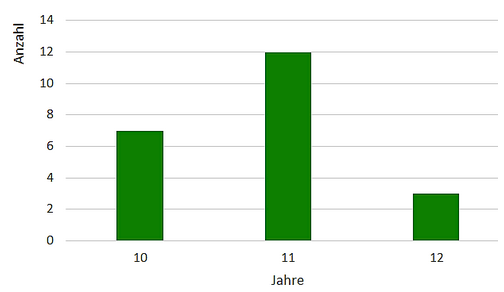
\includegraphics[width=70mm]{img/Grafik_A_Saeulendiagramm.png} &
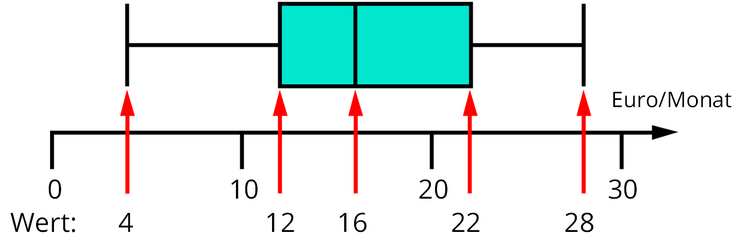
\includegraphics[width=70mm]{img/Grafik_B_Boxplot}\\
\hline
C: & D: \\
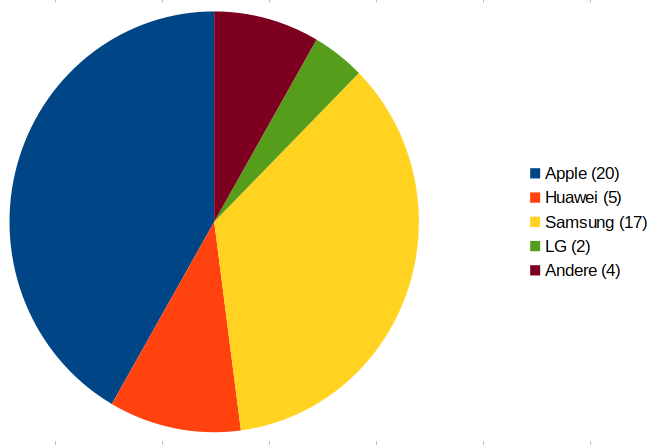
\includegraphics[width=70mm]{img/Grafik_C_Kreisdiagramm.png} &
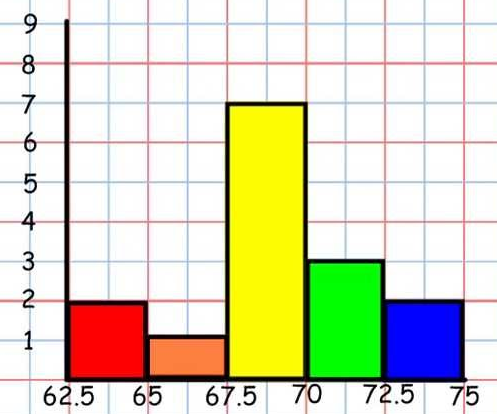
\includegraphics[width=70mm]{img/Grafik_D_Histogramm.png}
\end{tabular}


a) Um welche Art von Diagramm handelt es sich?
   (Auswahl: Balkendiagramm/Säulendiagramm, Kreisdiagramm, Boxplot, Histogramm)

A) \TRAINER{Balkendiagramm/Säulendiagramm}

B) \TRAINER{Boxplot}

C) \TRAINER{Kreisdiagramm}

D) \TRAINER{Histogramm}

\vspace{15mm}
\hrule

b) Handelt es sich um
nominale, ordinale oder kardinale (Intervalle/Verhältnisse) Daten?

A) \TRAINER{Ordinale oder diskretisierte kardinale}

B) \TRAINER{Kardinale}

C) \TRAINER{Nominale}

D) \TRAINER{Kardinale}


\vspace{15mm}
\hrule

c) Bestimmen Sie falls jeweils den Stichprobenumfang $n$:

A) \TRAINER{22}

B) \TRAINER{kann nicht bestimmt werden}

C) \TRAINER{48}

D) \TRAINER{15}


\vspace{15mm}
\hrule

d) Bestimmen Sie jeweils das Minimum:

A) \TRAINER{10}

B) \TRAINER{4}

C) \TRAINER{Es sind nur nominale Daten. Ein Minimum gibt es erst bei
ordinalen Daten. Alphabetisch ist natürlich «andere» das Minimum. Und
vom Vorkommen wäre es LG.}

D) \TRAINER{Sind nur kategorisierte Daten. Das Minimum zu bestimmen
ist somit unmöglich. Wir wissen nur, das Minimum liegt im Bereich 62.5
bis 65.}


\vspace{15mm}
\hrule

e) Bestimmen Sie den Mittelwert

A) \TRAINER{$10.\overline{81}$}

B) \TRAINER{nicht möglich, da klassierte Daten}

C) \TRAINER{nicht möglich, da nominale Daten nicht einmal geordnet
werden können.}

D) \TRAINER{Nicht möglich, da klassierte Daten. Wir wissen nicht wo
innerhalb der Säulen sich die Werte befinden.}


\vspace{15mm}
\hrule

f) Bestimmen Sie den Modus:

A) \TRAINER{11}

B) \TRAINER{nicht möglich}

C) \TRAINER{Apple}

D) \TRAINER{nicht möglich}



\vspace{15mm}
\hrule

g) Bestimmen Sie den Median:

A) \TRAINER{11}

B) \TRAINER{16}

C) \TRAINER{nicht möglich, da nur nominale Daten}

D) \TRAINER{nicht möglich, da klassifizierte Daten}

\newpage

h) Bestimmen Sie die Standardabweichung


A) \TRAINER{$\sigma=0.649220766,   S=0.664498639$}

B) \TRAINER{nicht möglich, da Boxplots immer klassifizierte Daten
angeben}

C) \TRAINER{nicht möglich für nominale Daten}

D) \TRAINER{nicht möglich für klassifizierte Daten}


\vspace{15mm}
\hrule


i) Bestimmen Sie die Quartilsdifferenz QD (= Interquartile Range IQR):

A) \TRAINER{1 (= 11-10)}

B) \TRAINER{10}

C) \TRAINER{nicht möglich für nominale Daten}

D) \TRAINER{nicht möglich für klassierte Daten}

\newpage





\end{document}
